\documentclass[aspectratio=169]{beamer}

\setbeamersize{text margin left=5mm, text margin right=5mm}

\defbeamertemplate{headline}{my header}{%
\vskip1pt%
\makebox[0pt][l]{\,\insertshortauthor}%
\hspace*{\fill}\insertshorttitle/\insertshortsubtitle\hspace*{\fill}%
\llap{\insertpagenumber/\insertpresentationendpage\,}
}
\setbeamertemplate{headline}[my header]

\let\olditem\item
\renewcommand{\item}{\setlength{\itemsep}{\fill}\olditem}

\usepackage{caption}
\usepackage{soul}
\usepackage{tkz-euclide}
\usetikzlibrary{calc}
\usepackage[]{algorithm2e}
\usepackage{changepage}
\usepackage{amssymb}
\usepackage{xcolor}
\usepackage{mathtools}
\usepackage{tcolorbox}
\usepackage{tikz}
\usepackage{tikz-3dplot}
\usepackage{tkz-euclide}
\usepackage{circuitikz}
\usepackage{mleftright}
\usetikzlibrary{arrows.meta, decorations.pathreplacing, positioning, shapes.geometric}
\usepackage[tikz]{bclogo}
\presetkeys{bclogo}{
    ombre=false,
    epBord=0,
    couleur = black!10!white,
    couleurBord = red,
    arrondi = 0.1,
    logo=,
}{}

%% Fonts
\usefonttheme{professionalfonts}
\usefonttheme{serif}

\DeclareCaptionLabelFormat{blank}{}
\captionsetup[figure]{labelformat=blank}

%% Math definitions
\def\mf{\ensuremath\mathbf}
\def\mb{\ensuremath\mathbb}
\def\mc{\ensuremath\mathcal}
\def\lp{\ensuremath\left(}
\def\rp{\ensuremath\right)}
\def\lv{\ensuremath\left\lvert}
\def\rv{\ensuremath\right\rvert}
\def\lV{\ensuremath\left\lVert}
\def\rV{\ensuremath\right\rVert}
\def\lc{\ensuremath\left\{}
\def\rc{\ensuremath\right\}}
\def\ls{\ensuremath\left[}
\def\rs{\ensuremath\right]}
\def\bmx{\ensuremath\begin{bmatrix*}[r]}
\def\emx{\ensuremath\end{bmatrix*}}
\def\bmxc{\ensuremath\begin{bmatrix*}[c]}
\def\t{\lp t\rp}
\def\k{\ls k\rs}

\newcommand{\demoex}[2]{\onslide<#1->\begin{color}{black!60} #2 \end{color}}
\newcommand{\demoexc}[3]{\onslide<#1->\begin{color}{#2} #3 \end{color}}
\newcommand{\anim}[3]{\onslide<#1->{\begin{color}{#2!60} #3 \end{color}}}
\newcommand{\ct}[1]{\lp #1\rp}
\newcommand{\dt}[1]{\ls #1\rs}
\newcommand{\cols}[2]{\begin{columns}[#1] #2 \end{columns}}
\newcommand{\col}[2]{\begin{column}{#1} #2 \end{column}}

%% Mycolors
\definecolor{myred}{RGB}{192,0,0}
\definecolor{mygray}{RGB}{100,100,100}

%% Custom beamer color
\setbeamercolor{title}{fg=myred}
\setbeamercolor{subtitle}{fg=myred}
\setbeamerfont{title}{series=\bfseries}
% \setbeamercolor{frametitle}{bg=myred, fg=white}
\setbeamercolor{frametitle}{bg=mygray!10!, fg=myred}
\setbeamerfont{frametitle}{series=\bfseries}
\setbeamercolor{item}{fg=mygray}
\setbeamercolor{title in head/foot}{fg=myred}

% Move header to footer
\setbeamertemplate{headline}{}
\setbeamertemplate{footline}{
  \begin{beamercolorbox}[wd=\paperwidth,ht=2.25ex,dp=1ex,center]{footline}
    \inserttitle\hfill\insertauthor\hfill\insertdate\hfill\insertframenumber{}
  \end{beamercolorbox}
}


\title{Applied Linear Algebra for Data}

% A subtitle is optional and this may be deleted
\subtitle{Application: Linear Dynamical Systems}

\author{Sivakumar Balasubramanian}
% - Give the names in the same order as the appear in the paper.
% - Use the \inst{?} command only if the authors have different
%   affiliation.

\institute[Christian Medical College] % (optional, but mostly needed)
{
  \inst{}%
  Department of Bioengineering\\
  Christian Medical College, Bagayam\\
  Vellore 632002
}
% - Use the \inst command only if there are several affiliations.
% - Keep it simple, no one is interested in your street address.

\date{}
% - Either use conference name or its abbreviation.
% - Not really informative to the audience, more for people (including
%   yourself) who are reading the slides online

\subject{Lecture notes on ALADA}
% This is only inserted into the PDF information catalog. Can be left
% out. 

% If you have a file called "university-logo-filename.xxx", where xxx
% is a graphic format that can be processed by latex or pdflatex,
% resp., then you can add a logo as follows:

% \pgfdeclareimage[height=0.5cm]{university-logo}{university-logo-filename}
% \logo{\pgfuseimage{university-logo}}

% Delete this, if you do not want the table of contents to pop up at
% the beginning of each subsection:
\AtBeginSubsection[]
{
  \begin{frame}<beamer>{Outline}
    \tableofcontents[currentsection,currentsubsection]
  \end{frame}
}

% Let's get started
\begin{document}

% \pgfplotsset{
%   compat=1.8,
%   colormap={whitered}{color(0cm)=(white); color(1cm)=(orange!75!red)}
% }


\begin{frame}
  \titlepage
\end{frame}


\begin{frame}{Linear System}
\begin{center}
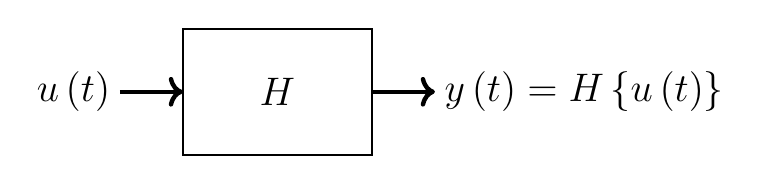
\begin{tikzpicture}[scale=0.8]
    \draw[thick] (0,0) rectangle (3, 2);
    \node at (1.5, 1) {{\Large $H$}};
    \draw[ultra thick, ->] (-1, 1) -- (0, 1);
    \node[left] at (-1, 1) {{\Large $u\lp t\rp$}};
    \draw[ultra thick, ->] (3, 1) -- (4, 1);
    \node[right] at (4, 1) {{\Large $y\lp t\rp = H\lc u\lp t\rp\rc$}};
\end{tikzpicture}
\end{center}

Behavior of dynamic systems can be described mathematically through differential equations (continuous-time systems), or difference equations (discrete-time systems).
\vspace{0.25cm}

A system is \textbf{linear} iff, 
\[ y_1\lp t\rp = H\lc u_1\lp t\rp\rc \text{ and } y_2\lp t\rp = H\lc u_2 \lp t\rp \rc\]
\[ \begin{split}
    \implies H\lc a_1x_1\lp t\rp + a_2u_2\lp t\rp \rc &= a_1H\lc u_1\lp t\rp\rc + a_2H\lc u_2\lp t\rp \rc\\
    &= a_1y\lp t\rp + a_2y_2\lp t\rp, \, a_1, a_2 \in \mathbb{C}
\end{split}
\]
\end{frame}


\begin{frame}{Time-Invariant System}
\begin{center}
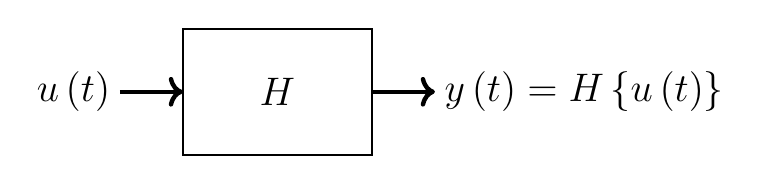
\begin{tikzpicture}[scale=0.8]
    \draw[thick] (0,0) rectangle (3, 2);
    \node at (1.5, 1) {{\Large $H$}};
    \draw[ultra thick, ->] (-1, 1) -- (0, 1);
    \node[left] at (-1, 1) {{\Large $u\lp t\rp$}};
    \draw[ultra thick, ->] (3, 1) -- (4, 1);
    \node[right] at (4, 1) {{\Large $y\lp t\rp = H\lc u\lp t\rp\rc$}};
\end{tikzpicture}
\end{center}
\begin{itemize}
    \item A system is \textbf{time-invariant} if,
    \[ y\lp t\rp = H\lc u\lp t\rp\rc \implies H\lc u \lp t - \tau \rp \rc = y\lp t - \tau \rp \]

    \item Characteristics of the system do not change with time. Time-shifted inputs produce correspondingly time-shifted output.
\end{itemize}
\end{frame}


\begin{frame}{Linear Time-Invariant System}
    \vspace{-0.5cm}
\begin{center}
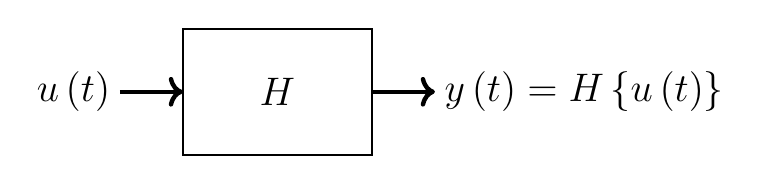
\begin{tikzpicture}[scale=0.8]
    \draw[thick] (0,0) rectangle (3, 2);
    \node at (1.5, 1) {{\Large $H$}};
    \draw[ultra thick, ->] (-1, 1) -- (0, 1);
    \node[left] at (-1, 1) {{\Large $u\lp t\rp$}};
    \draw[ultra thick, ->] (3, 1) -- (4, 1);
    \node[right] at (4, 1) {{\Large $y\lp t\rp = H\lc u\lp t\rp\rc$}};
\end{tikzpicture}
\end{center}

LTI systems: both \textbf{linear} and \textbf{time-invariant}. These are described through constant coefficient linear differential (or difference) equations.


\textbf{Continuous-time}: 
$$\frac{d^n}{dt^n}y\lp t\rp + a_{1}\frac{d^{n-1}}{dt^{n-1}}y\lp t\rp + \ldots + a_ny\lp t\rp = u\lp t\rp + b_1\frac{d}{dt}u\lp t\rp + \ldots + b_m\frac{d^m}{dt^m}y\lp t\rp $$


\textbf{Discrete-time}:
$$y\ls k - n\rs + a_1y\ls k - n + 1\rs + \ldots + a_ny\ls k\rs = u\ls k\rs + b_1u\ls k-1\rs + \ldots + b_m u\ls k-m\rs$$
\end{frame}


\begin{frame}[t]{State space representation of linear systems}
    \begin{itemize}
        \item In the case of a linear system, the equations representing the dynamics takes a simpler form,
        \[ \dot{\mf{x}}\ct{t} = \mf{A}\ct{t}\mf{x}\ct{t} + \mf{B}\ct{t}\mf{u}\ct{t} \]
        \[ \mf{y}\ct{t} = \mf{C}\ct{t}\mf{x}\ct{t} + \mf{D}\ct{t}\mf{u}\ct{t} \]
        where,\\
        $\bullet \quad $ $\mf{A}\ct{t} \in \mb{R}^{n \times n}$ is the \textit{system} matrix.\\
        $\bullet \quad $ $\mf{B}\ct{t} \in \mb{R}^{n \times p}$ is the \textit{input} matrix.\\
        $\bullet \quad $ $\mf{C}\ct{t} \in \mb{R}^{m \times n}$ is the \textit{output} matrix.\\
        $\bullet \quad $ $\mf{D}\ct{t} \in \mb{R}^{m \times p}$ is the \textit{feedforward}matrix.
    \end{itemize}
\end{frame}
    
    
\begin{frame}[t]{State space representation of linear systems}
\begin{itemize}
    \item In the case of time-invariant system, the matrices are constant.
    \[ \dot{\mf{x}}\ct{t} = \mf{A}\mf{x}\ct{t} + \mf{B}\mf{u}\ct{t} \]
    \[ \mf{y}\ct{t} = \mf{C}\mf{x}\ct{t} + \mf{D}\mf{u}\ct{t} \]

    \item These two equations represent how the states and the measured outputs of the system are affected by the current states and inputs. The individual terms in these matrices indicate how a particular state/input affects another state/output.
\end{itemize}
\end{frame}


\begin{frame}{State space representation of discrete-time linear systems}
\begin{itemize}
    \item Discrete-time linear system,
    \[ \mf{x}\dt{k+1} = \mf{A}\dt{k}\mf{x}\dt{k} + \mf{B}\dt{k}\mf{u}\dt{k} \]
    \[ \mf{y}\dt{k} = \mf{C}\dt{k}\mf{x}\dt{k} + \mf{D}\dt{k}\mf{u}\dt{k} \]
    where, $k \in \mb{Z}$ correspond to time index.
    \begin{itemize}
        \item $\mf{A}\dt{k} \in \mb{R}^{n \times n}$ is the \textit{system} matrix.
        \item $\mf{B}\dt{k} \in \mb{R}^{n \times p}$ is the \textit{input} matrix.
        \item $\mf{C}\dt{k} \in \mb{R}^{m \times n}$ is the \textit{output} matrix.
        \item $\mf{D}\dt{k} \in \mb{R}^{m \times p}$ is the \textit{feedforward} matrix.
    \end{itemize}

    \item In the case of time-invariant system, the matrices are constant.
    \[ \mf{x}\dt{k+1} = \mf{A}\mf{x}\dt{k} + \mf{B}\mf{u}\dt{k} \]
    \[ \mf{y}\dt{k} = \mf{C}\mf{x}\dt{k} + \mf{D}\mf{u}\dt{k} \]
\end{itemize}
\end{frame}


\begin{frame}[t]{Zero-input solution for $\mf{x}\ct{t}$}
\begin{itemize}
    \item \textbf{Zero-Input Solution}: We will start by assuming $\mf{u}\ct{t} = \mf{0}$.
    \[ \dot{\mf{x}}\ct{t} = \mf{A}\mf{x}\ct{t} \]
    And that the initial value of the state at time $t = 0^-$ is $\mf{x}\ct{0^-} = \mf{x}_0$. 

    \item The solution to this differential equation is given by,
    \[ \mf{x}\ct{0} = e^{t\mf{A}}\mf{x}_0, \,\, t \geq 0 \]
    where, $e^{t\mf{A}}$ is the matrix exponential of $\mf{A}$.

    \item Note the interesting similarity to the scalar case: $\dot{x}\ct{t} = ax\ct{t}$, we know the solution to be the following, $x\ct{t} = e^{at}x\ct{0^-}$. 
\end{itemize}
\end{frame}


\begin{frame}[t]{What is the matrix exponential $e^{t\mf{A}}$?}
\begin{itemize}
    \item Functions of matrices are often defined to have properties consistent with that of their scalar coutnerparts. 
    \[ e^{t\mf{A}} = \mf{I} + t\mf{A} + \frac{1}{2!}t^2\mf{A}^2 + \ldots = \sum_{k=0}^{\infty} \frac{1}{k!}t^k\mf{A}^k \implies \frac{d}{dt}e^{t\mf{A}} = \mf{A}e^{t\mf{A}} \]
    
    \item But we do not have to compute all the powers of $\mf{A}$ to compute the matrix exponential. Thanks to the Cayley-Hamilton theorm,
    
    \begin{bclogo}{Cayley-Hamilton Theorem}
    Every square matrix $\mf{A} \in \mb{R}^{n \times n}$ satisfies it own characteristic equation $p\lp \lambda \rp = 0$, i.e. $p\lp\mf{A}\rp = \mf{0}$.
    \[ p\lp\mf{A}\rp = \mf{A}^n + a_1\mf{A}^{n-1} + a_2\mf{A}^{n-2} + \ldots + a_n\mf{I} = \mf{0} \]
    \end{bclogo}

\end{itemize}
\end{frame}


\begin{frame}[t]{What is the matrix exponential $e^{t\mf{A}}$?}
\begin{itemize}
    \item $e^{t\mf{A}}$ can be computed as the following,
    \[e^{t\mf{A}} = \sum_{k=0}^{n-1} c_kt\mf{A}^k \]
    
    \item When the matrix $\mf{A}$ is diagonalizable, then the matrix exponential can be computed as follows,
    \[\begin{split}
        e^{t\mf{A}} &= \sum_{k=0}^{n-1} c_kt^k\mf{A}^k = \sum_{k=0}^{n-1} c_kt^k\ct{\mf{V}\mf{\Lambda}\mf{V}^{-1}}^k \\
        &= \sum_{k=0}^{n-1} c_kt\mf{V}\mf{\Lambda}^k\mf{V}^{-1} = = \mf{V}\ct{\sum_{k=0}^{n-1} c_kt\mf{\Lambda}^k}\mf{V}^{-1}\\
        &= \mf{V}e^{t\mf{\Lambda}}\mf{V}^{-1}\\
    \end{split}
    \]
\end{itemize}
\end{frame}


\begin{frame}[t]{Usefulness of the $e^{t\mf{A}}$?}
\begin{itemize}
    \item Let $\lc \ct{\lambda_i, \mf{v}_i} \rc_{i=1}^n$ be the $n$ eigenpairs of the matrix $\mf{A}$. Then, 
    \[ e^{t\mf{\Lambda}} = \bmxc
    e^{t \lambda_1} & 0 & 0 & \cdots & 0\\
    0 & e^{t \lambda_2} & 0 & \cdots & 0\\
    \vdots & \vdots & \vdots & \ddots & \vdots\\
    0 & 0 & 0 & \cdots & e^{t\lambda_n}
    \emx\]
    \[ e^{t\mf{A}} = \mf{V}e^{t\mf{\Lambda}}\mf{V}^{-1} \]
    
    The eigenvectors in this case are referred to the as the eigenmodes of the system, which are a characteristic of the system. The eigenvalues are the corresponding rates of exponential growth/decay of the eigenmodes.

    \item The reprsentation allows us to express the response to any initial condition as the linear combination of the exponential evolution of the eigenmodes.
\end{itemize}
\end{frame}


\begin{frame}[t]{Usefulness of the $e^{t\mf{A}}$}
\begin{itemize}
    \item Let $\mf{x}_0$ is the initial state at time $t = 0^-$. Then the zero-input response can be expressed as the following,
    \[ \mf{x}\ct{t} = \mf{V}e^{t\mf{\Lambda}}\mf{V}^{-1}\mf{x}_0 \]
    
    We know, $\mf{V} = \bmx \mf{v}_1 & \mf{v}_2 & \cdots & \mf{v}_n\emx$, and let $\mf{V}^{-1} = \bmx \tilde{\mf{v}}_1^\top \\ \tilde{\mf{v}}_2^\top \\ \vdots \\ \tilde{\mf{v}}_n^\top \emx$.
    
    Then we can expressed the above expression as,
    \[ \mf{x}\ct{t} = \sum_{i=1}^n e^{t \lambda_i} \mf{v}_i\tilde{\mf{v}}_i^\top \mf{x}_0 \]

    $\mf{v}_i\tilde{\mf{v}}_i^\top \mf{x}_0$ is the projection of the initial state $\mf{x}_0$ onto the $i$-th eigenmode. The exponential term $e^{t \lambda_i}$ is the rate of exponential growth/decay of the $i$-th eigenmode.
\end{itemize}
\end{frame}


\begin{frame}[t]{Solution for discrete-time LTI system}
\begin{itemize}
    \item \textbf{System equations}:
    \[ \mf{x}\dt{k+1} = \mf{A}\mf{x}\dt{k} + \mf{B}\mf{u}\dt{k} \]
    \[ \mf{y}\dt{k} = \mf{C}\mf{x}\dt{k} + \mf{D}\mf{u}\dt{k} \]

    \item \textbf{Zero-input solution}:
    $$\mf{x}\dt{k} = \mf{A}^k\mf{x}\dt{0}$$
    
    \item If $\mf{A}$ is diagonalizable, then,
    $$\mf{x}\dt{k} = \mf{V}\mf{\Lambda}^k\mf{V}^{-1}\mf{x}\dt{0}$$
\end{itemize}
\end{frame}

\begin{frame}[t]{Internal stability}
\begin{itemize}
    \item There are two types of stability one can associate with a system  -- \textbf{Internal stability} and \textbf{Input-Output stability}.

    \item \textbf{Internal stability}: Deals with the stability of the zero-input response of the system states.
\end{itemize}
\end{frame}


\begin{frame}[t]{Internal stability}
\begin{itemize}
    \item Definition of stability in the Lyapunov sense for linear systems: 
    \begin{itemize}
        \item The zero-input response of a linear system $\dot{\mf{x}}\ct{t} = \mf{A}\mf{x}\ct{t}$ is \textit{stable or marginally stable} if every finite initial condition $\mf{x}\ct{0^-}$ results in a bounded state trajectory $\mf{x}\ct{t}$ $\forall t \geq 0$.
        \[ \lV \mf{x}\ct{t}\rV \leq d, \,\,\, \forall t \geq 0 \]

        \item The zero-input response is \textit{asymtotically stable} if everyf initial condition $\mf{x}\ct{0^-}$ results in a bounded state trajectory $\mf{x}\ct{t}$ that coverges to $0$ as $t \to \infty$.
        \[ \lV \mf{x}\ct{t}\rV \leq d \text{ and } \lim_{t \to \infty} \lV \mf{x}\ct{t}\rV = 0 \]
    \end{itemize}
\end{itemize}
\end{frame}


\begin{frame}[t]{Internal stability}
\begin{itemize}
    \item The system $\dot{\mf{x}}\ct{t} = \mf{A}\mf{x}\ct{t}$ is marginally stable if and only if all eigenvales of $\mf{A}$ have either zero or negative real parts, and the eigenvalues with zero real parts have the same algebraic and geometric multiplicity.

    \item  The system $\dot{\mf{x}}\ct{t} = \mf{A}\mf{x}\ct{t}$ is asymptotically stable if and only if all eigenvales of $\mf{A}$ have  negative real parts.
\end{itemize}
\end{frame}


\begin{frame}[t]{Internal stability}
\begin{itemize}
    \item Consider the solution, $\mf{x}\ct{t} = e^{t\mf{A}}\mf{x}\ct{0^-}, \,\,\, t \geq 0$, and $\mf{A} = \mf{V}\mf{J}\mf{V}^{-1}$.
    \[ \lV \mf{x}\ct{t} \rV = \lV e^{t\mf{A}}\mf{x}\ct{0^-} \rV \leq \lV e^{t\mf{J}} \rV \lV \mf{x}\ct{0^-} \rV\]

    \item When $\mf{A}$ is diagonalizable ($\lambda_i$ are the eigenvalues of $\mf{A}$),
    \begin{itemize}
        \item $ \lV \mf{x}\ct{t} \rV \leq  e^{\sigma t} \lV \mf{x}\ct{0^-} \rV$, where $\sigma = \max_i \Re \lc \lambda_i \rc$.
        \item When $\sigma = 0$, $\lV \mf{x}\ct{t}\rV$ is bounded $\forall t \geq 0$.
        \item When $\sigma < 0$, $\lim_{t \to \infty} \lV \mf{x}\ct{t}\rV = 0$.
    \end{itemize}\vspace{0.2cm}
\end{itemize}
\end{frame}


\begin{frame}[t]{Internal stability -- Discrete-time LTI systems}
When $\mf{A}$ is diagonalizable ($\lambda_i$ are the eigenvalues of $\mf{A}$),
\begin{itemize}
    \item $\lV \mf{x}\dt{k} \rV \leq  \lv \lambda \rv^k \lV \mf{x}\dt{0} \rV$, where $\lambda = \max_i \lv \lambda_i \rv$.
    \item When $\lv \lambda \rv = 1$, $\lV \mf{x}\dt{k}\rV$ is bounded $\forall k > 0$.
    \item When $\lv \lambda \rv < 1$, $\lim_{k \to \infty} \lV \mf{x}\dt{k}\rV = 0$.
\end{itemize}
\end{frame}
    
    
\end{document}